\chapter{Results} \label{sec:results}

The performance of the device was analyzed by measuring some resistors and other mixed networks.

With small resistors in the range of a few \unit{10}{\ohm} to \unit{10}{\kilo\ohm}, the accuracy is better than
\unit{1}{\%}.
\autoref{fig:meas_49r9} shows a measurement of a \unit{49.9}{\ohm} resistor,
\autoref{fig:meas_5k6} shows the results with a \unit{5.6}{\kilo\ohm} resistor
and \autoref{fig:meas_10k} the results with a \unit{10}{\kilo\ohm} resistor.
Every profile is well within the \unit{\pm 1}{\%} range, the impedance angle is close to 0 as would be expected from
an ohmic resistor.

For resistors of larger magnitude, the accuracy is not as good, a measurement of a \unit{1}{\mega\ohm} resistor can be
seen in \autoref{fig:meas_1M}. There are non-linear terms in the system gain that are not compensated by the two-point
calibration, which result in the nonlinear impedance profile. The measured angle shows a linear trend, which should
be compensated by the two-point calibration but is not.
Also note the change in slope and noise at \unit{10}{\kilo\hertz}, where the clock source is switched from the external
source below \unit{10}{\kilo\hertz} to the internal one above.

When sweeping over larger frequency ranges, the accuracy is not as good, especially in the range near or above
\unit{100}{\kilo\hertz}.
In general, it is advisable to use a frequency range as narrow as possible, since the two-point calibration can only
account for constant and linear terms in the system gain. Nonlinearities however only manifest when a large frequency
range is swept all at once.

For small mixed impedance networks however, the results are quite bad. Because of  an instability in the external AFE,
the measurement results cannot be used at all. \autoref{fig:meas_S22} shows a measurement of a high-Q LC resonant
circuit, as can be seen the impedance value as well as the resonant frequency of the circuit are way off.
A similar LC circuit with a lower Q-factor shows better results (compare \autoref{fig:meas_LCP}), the accuracy is not
good enough nonetheless.

A goal for further work on the device is to replace the current topology of the external analog front end
(inverting amplifier configured as an attenuator on the output, current to voltage conversion on the input)
by a different one. A possible approach is to use a current source on the output and directly measure the voltage
across the impedance on the input.

\begin{figure}[htpb]
  \centering
    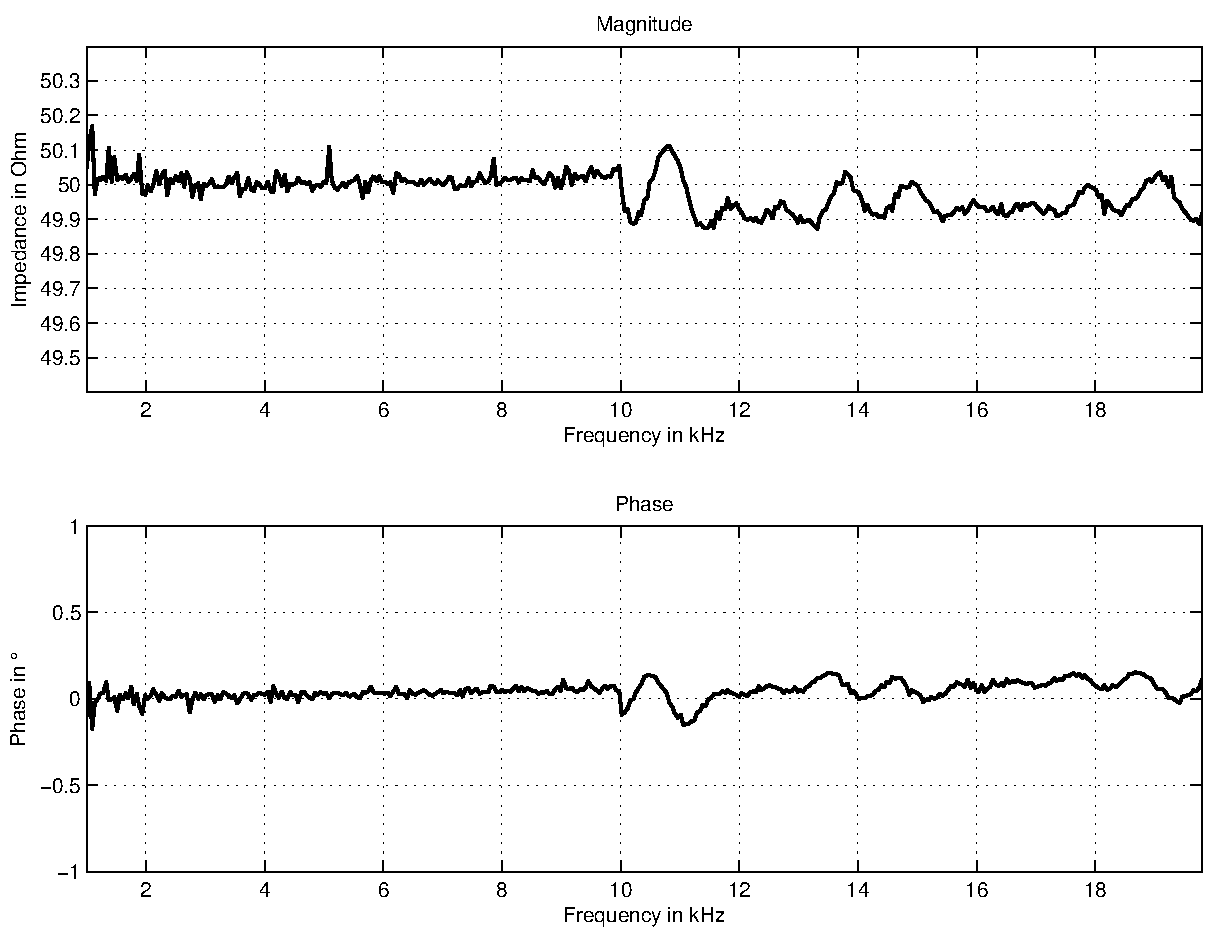
\includegraphics[width=0.9\textwidth]{bilder/meas_49r9.pdf}
  \caption{Measurement results of a \unit{49.9}{\ohm} resistor (with an actual value of about \unit{50}{\ohm}).
    The displayed magnitude range is \unit{\pm 1}{\%}.}
  \label{fig:meas_49r9}
\end{figure}

\begin{figure}[htpb]
  \centering
    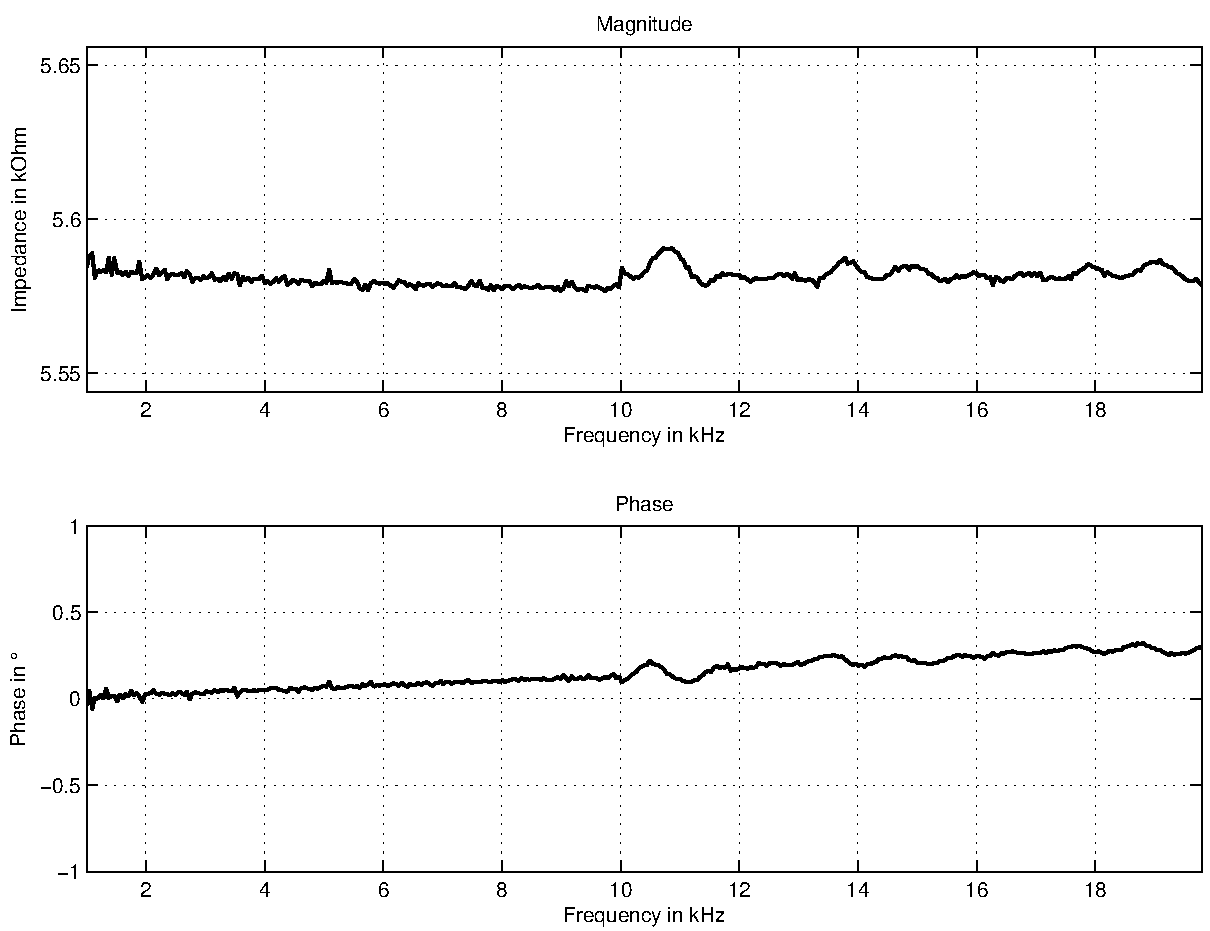
\includegraphics[width=0.9\textwidth]{bilder/meas_5k6.pdf}
  \caption{Measurement results of a \unit{5.6}{\kilo\ohm} resistor (with an actual value of about \unit{5.58}{\kilo\ohm}).
    The displayed magnitude range is \unit{\pm 1}{\%}.}
  \label{fig:meas_5k6}
\end{figure}

\begin{figure}[htpb]
  \centering
    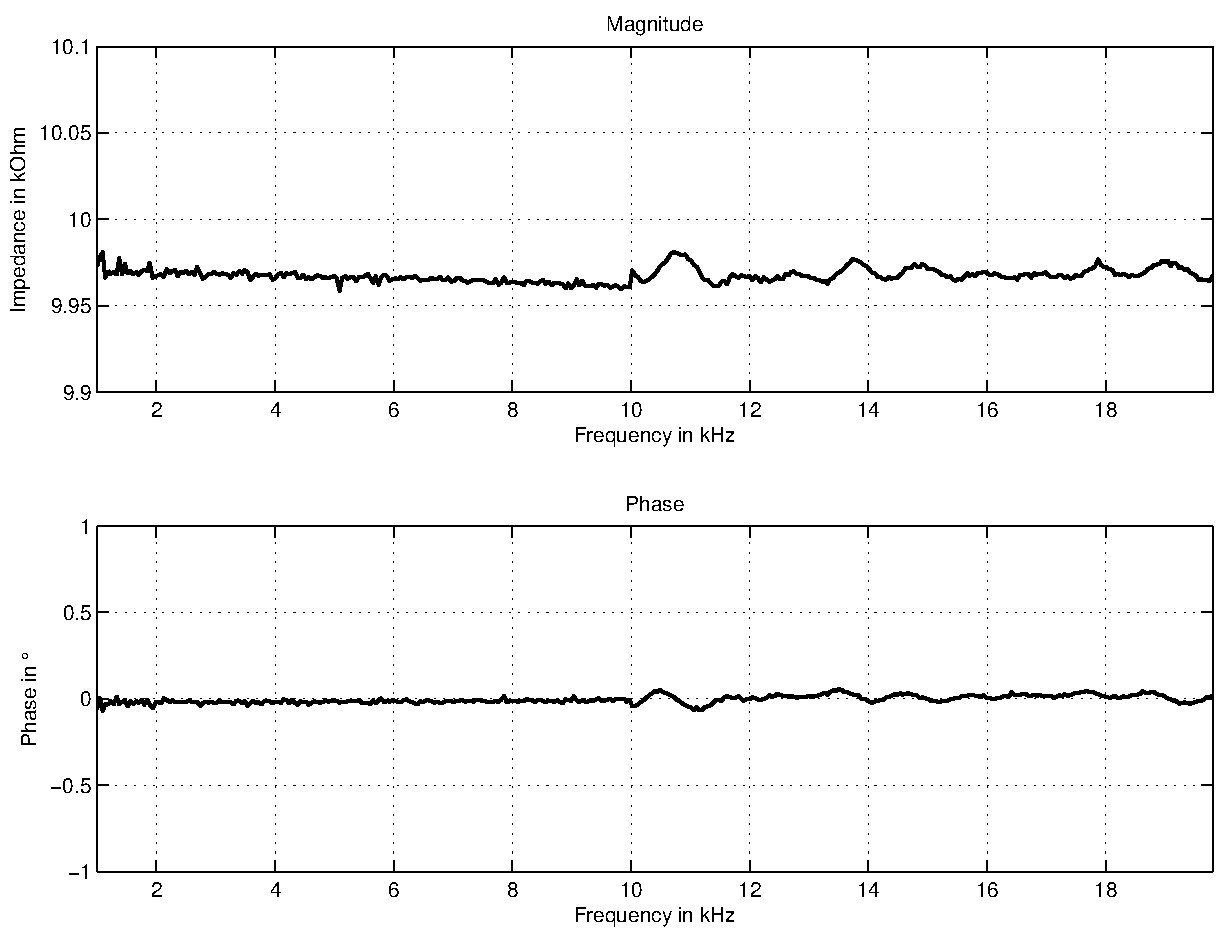
\includegraphics[width=0.9\textwidth]{bilder/meas_10k.pdf}
  \caption{Measurement results of a \unit{10}{\kilo\ohm} resistor (with an actual value of about \unit{9.96}{\kilo\ohm}).
    The displayed magnitude range is \unit{\pm 1}{\%}.}
  \label{fig:meas_10k}
\end{figure}

\begin{figure}[htpb]
  \centering
    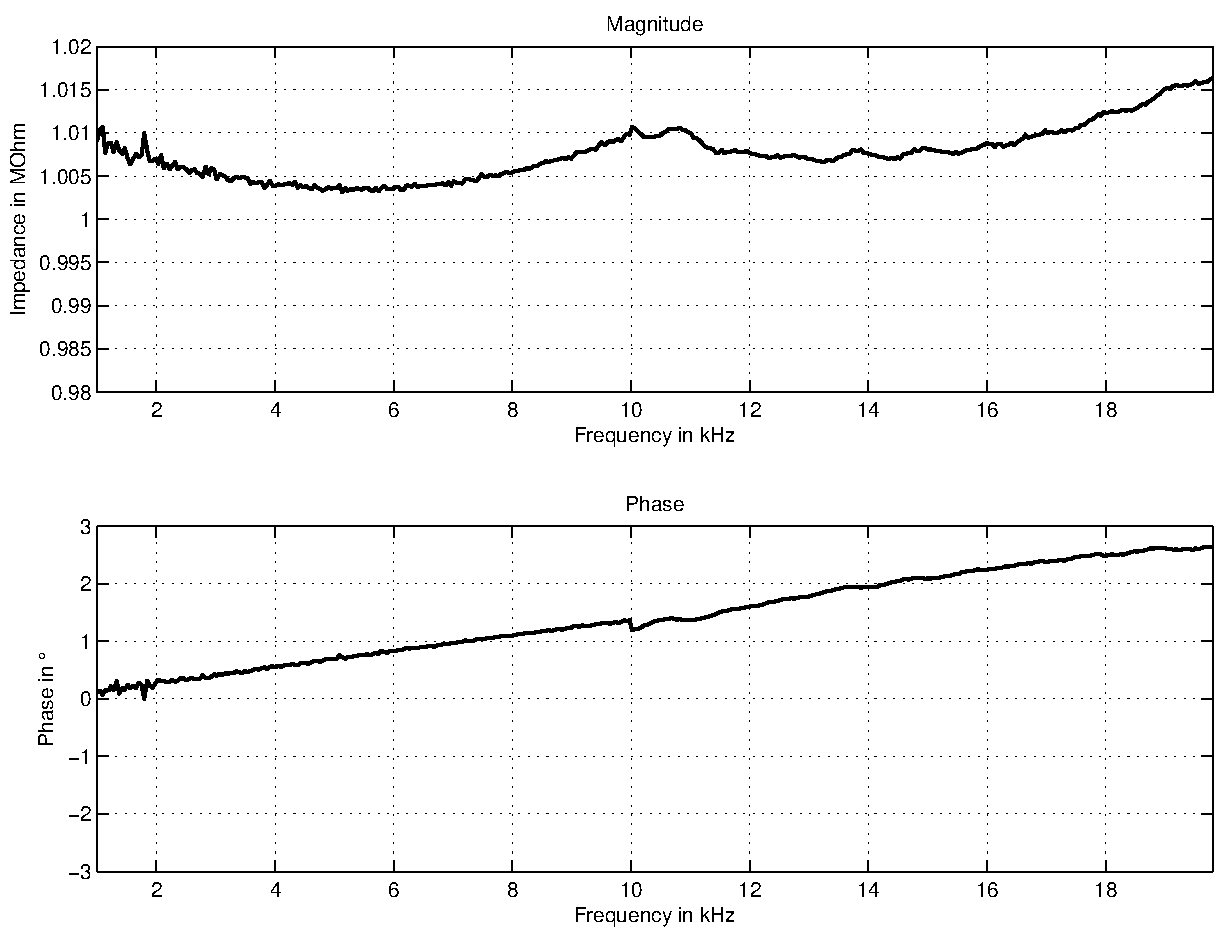
\includegraphics[width=0.9\textwidth]{bilder/meas_1M.pdf}
  \caption{Measurement results of a \unit{1}{\mega\ohm} resistor (with an actual value of about \unit{1}{\mega\ohm}).
    The displayed magnitude range is \unit{\pm 2}{\%}.}
  \label{fig:meas_1M}
\end{figure}

\begin{figure}[htpb]
  \centering
    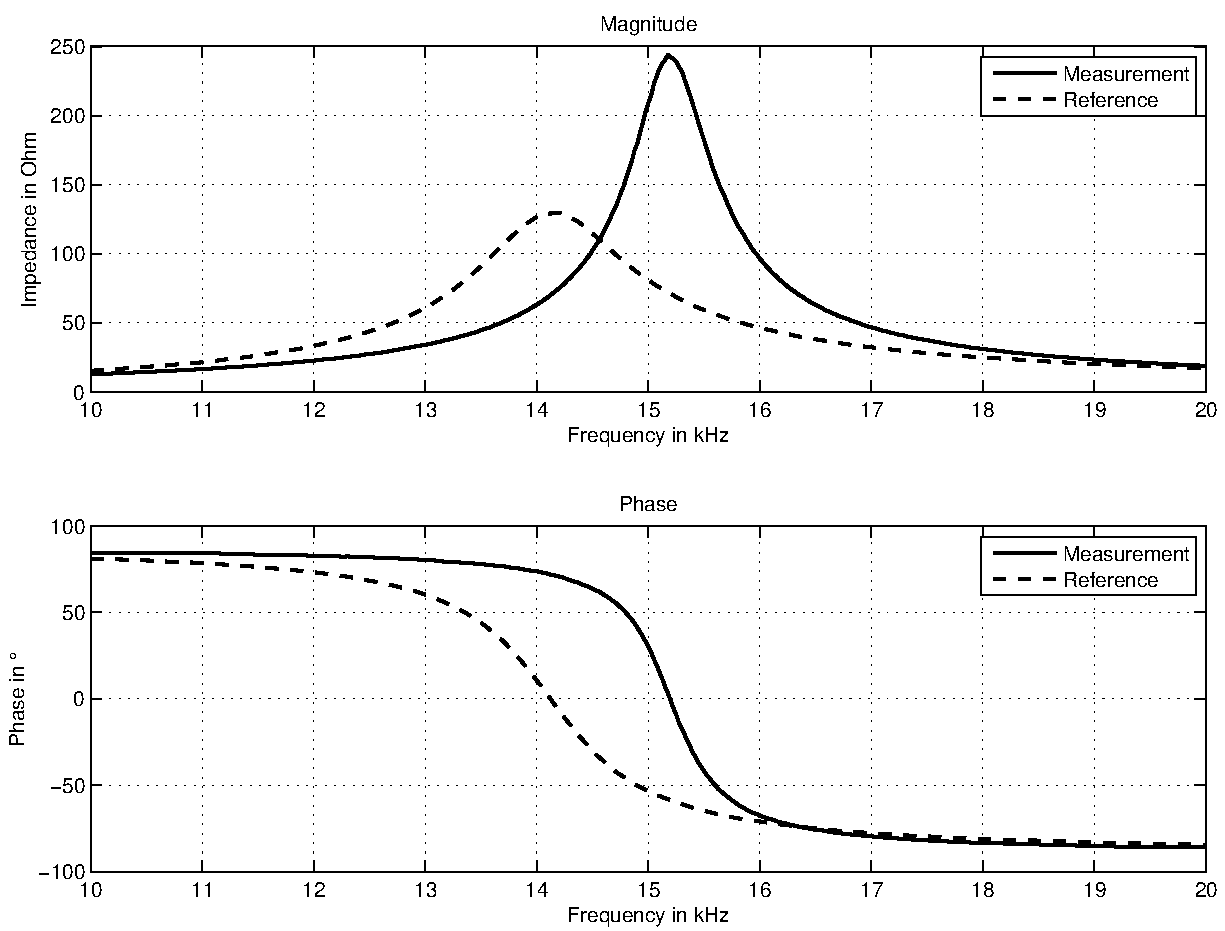
\includegraphics[width=0.9\textwidth]{bilder/meas_S22.pdf}
  \caption{Measurement results of a high-Q LC resonant circuit ($ \unit{1}{\micro\farad} \,\|\, \unit{100}{\micro\henry} $).
    The solid line represents the measured value, the dashed line the actual impedance obtained from an Agilent 4294A
    impedance analyzer. }
  \label{fig:meas_S22}
\end{figure}

\begin{figure}[htpb]
  \centering
    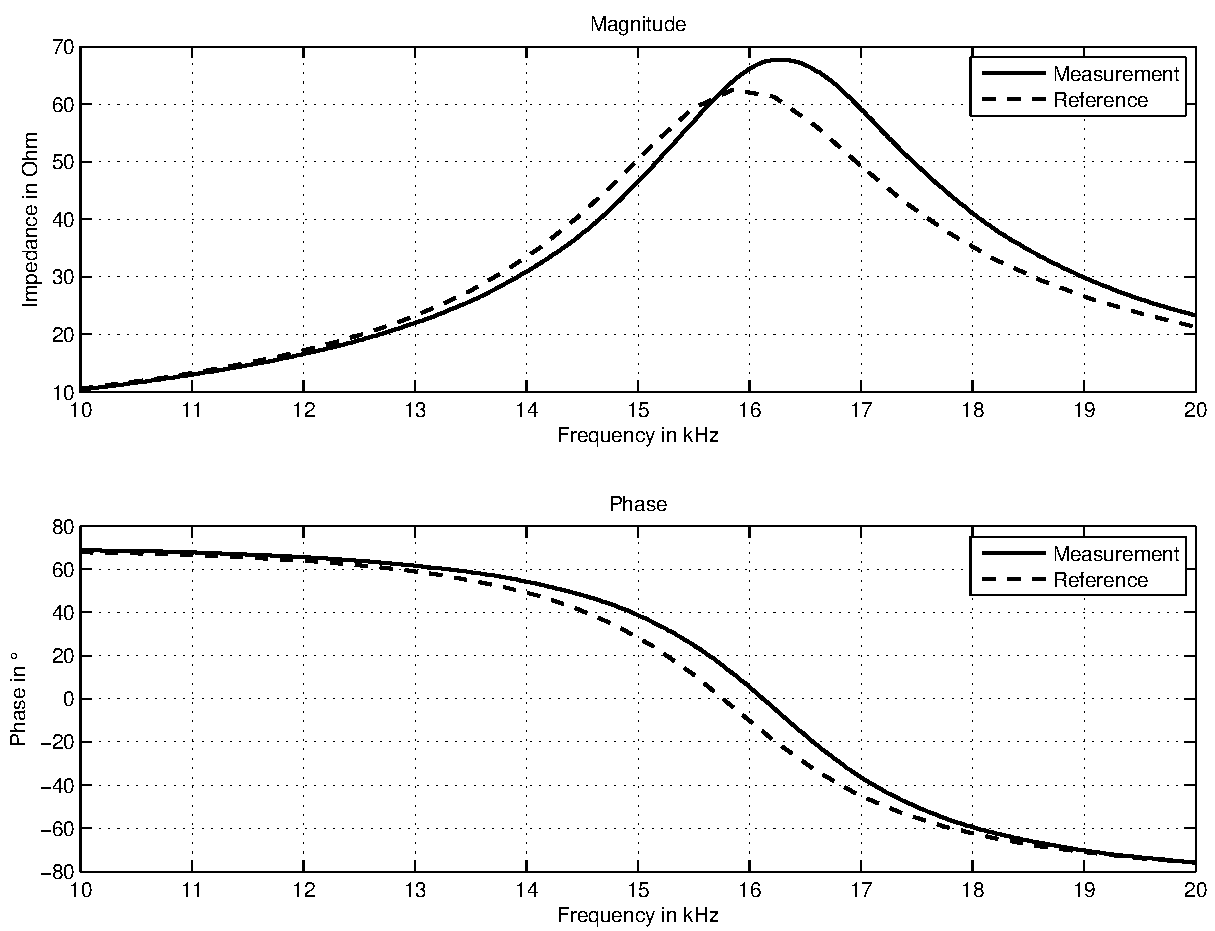
\includegraphics[width=0.9\textwidth]{bilder/meas_LCP.pdf}
  \caption{Measurement results of a low-Q LC resonant circuit ($ \unit{1}{\micro\farad} \,\|\, \unit{100}{\micro\henry} $).
    The solid line represents the measured value, the dashed line the actual impedance obtained from an Agilent 4294A
    impedance analyzer. }
  \label{fig:meas_LCP}
\end{figure}
